\documentclass[11pt]{article}

\usepackage[utf8]{inputenc}
\usepackage[T1]{fontenc}
\usepackage[margin=1in]{geometry}
\usepackage{booktabs}
\usepackage{tabularx}
\usepackage{graphicx}
\usepackage{enumitem}
\usepackage{hyperref}
\usepackage{xcolor}
\usepackage{parskip}

\setlength{\parskip}{6pt}
\renewcommand{\arraystretch}{1.25}

\newcolumntype{Y}{>{\raggedright\arraybackslash}X}

\newcommand{\placeholder}[1]{%
  \begin{center}
    \fbox{\parbox[c][2.6cm][c]{0.85\textwidth}{\centering\itshape #1}}
  \end{center}
}

\newcommand{\bracket}[1]{\textcolor{gray!70!black}{[#1]}}

\title{}
\date{}

\begin{document}
\pagestyle{plain}

\begin{center}
  {\LARGE \bfseries RAHEE} \\[4pt]
  {\Large Weekly Project Progress Report} \\[6pt]
  Week ending: 25 September 2026 \\
  Current progress: Single-device prototype complete; online multiplayer architecture designed
\end{center}

\vspace{8pt}

\begin{tabularx}{\textwidth}{@{} l Y @{}}
  \toprule
  \textbf{Project} & RAHEE --- an online digital version of a travel board game \\
  \textbf{Team size} & 5 members \\
  \textbf{Current stage} & Single-device (hotseat) prototype complete; design finalized for the real-time, multi-device online architecture; server implementation starting \\
  \textbf{Report purpose} & Weekly progress + implementation evidence \\
  \bottomrule
\end{tabularx}

\section{Project Overview}

RAHEE is a digital version of an existing travel board game by the Centre for Creative Learning (CCL), IIT Gandhinagar, in which two to six players travel across a map of India, spending a hand of playing cards as their itinerary, a fixed budget as they move, and scoring by visiting tourist places, reaching character-specific destinations, and collecting themed memory tokens.

The project's core requirement is that the game be \emph{data-driven}: the board --- cities, routes, route types, characters, destination goals, prices and scoring values --- is stored in a single structured data file and read by the game's rules engine at load time, so the engine itself contains no hard-coded board knowledge. A single-device (hotseat) version of the game, implementing this data-driven engine in full against the official rulebook, has been completed. The current implementation goal is extending this into a real-time, secure, multi-device online game, in which every player connects and plays from their own device, with public and private chat, as specified in the project's signed requirements sheet.

Current evidence covers the data-driven board setup, the rules engine, the single-device gameplay loop, its automated test suite, and the finalized design for the online multiplayer architecture.

\section{Current Architecture}

\begin{tabularx}{\textwidth}{@{} l l Y @{}}
  \toprule
  \textbf{Layer} & \textbf{Component} & \textbf{Purpose} \\
  \midrule
  Frontend & Plain JavaScript modules + SVG board & Map, tokens, hand, budget, memories, scoreboard views \\
  Rules engine & A single dependency-free JavaScript module & Dealing, movement, costs, memories, tourism, road trips, Aces, end-trigger, scoring --- no board knowledge of its own \\
  Board data & A structured JSON data file & The entire board: 101 cities, 209 routes, 6 characters (36 destination goals), full pricing and scoring table \\
  Backend \bracket{planned} & Node.js, Express, Socket.IO & Authoritative game rooms; real-time state, chat, over WebSocket \\
  Persistence \bracket{planned} & SQLite (embedded, file-based) & Save/resume of games in progress \\
  QA & Automated random-game simulation + headless-browser walkthroughs & Verify rule invariants and that a full game plays correctly end to end \\
  \bottomrule
\end{tabularx}

\textbf{Flow (current, single device):} Player $\rightarrow$ browser UI $\rightarrow$ rules engine (in-browser) $\rightarrow$ board data file $\rightarrow$ UI update.

\textbf{Flow (planned, online):} Player device $\rightarrow$ browser client $\rightarrow$ WebSocket $\rightarrow$ server (room + rules engine, authoritative) $\rightarrow$ per-player redaction $\rightarrow$ broadcast back to every connected device.

\section{Work Completed To Date}

\begin{itemize}[leftmargin=1.4em]
  \item Initial project setup: a dependency-free, browser-based application created (plain ES modules, no build step).
  \item Project repository and team development structure established.
  \item The full board encoded as a single structured data file: 101 cities, 209 routes (road, flight and ferry), 51 tourist places, 6 characters with 36 destination goals, and the complete pricing and scoring table.
  \item Rules engine implemented against the official rulebook, with no hard-coded board knowledge: dealing per player count, card-based movement, travel costs and surcharges, the four memory suits, tourist-place visits, road trips (invitation, shared cost, shared tourism, drop-off), all three uses of an Ace, the end-game trigger, and full scoring.
  \item Board rendered from the data file over the supplied map artwork: pan/zoom, routes, player tokens, and legal-move highlighting.
  \item Single-device (hotseat) game loop complete: setup, private handover between turns, turn actions, and a final scoreboard with a transparent score breakdown.
  \item Save and resume implemented for an in-progress single-device game.
  \item Automated test suite: full random-game simulation checking deck composition, rule invariants (no over-length move, spending only increases, no tourist place visited twice by one player, correct end-trigger and equal turn counts) and the rulebook's own worked examples; a separate headless-browser walkthrough drives a full game through real pointer input.
  \item Design finalized for the real-time, multi-device online architecture: client--server split, WebSocket transport, per-player server-side state redaction (so hands and in-progress route plans stay private), room-based sessions, and public/private chat.
\end{itemize}

\section{Screenshot Evidence}

Use the slots below in this order; each may also serve as a figure number in the final report. If a feature is not yet implemented, the slot is left blank rather than filled with a screenshot from an unrelated step.

\subsection*{S1 --- Project folder in editor}
\placeholder{PASTE SCREENSHOT HERE --- the Rahee project opened in an editor, showing the main folders and files}

\subsection*{S2 --- Application running}
\begin{center}
  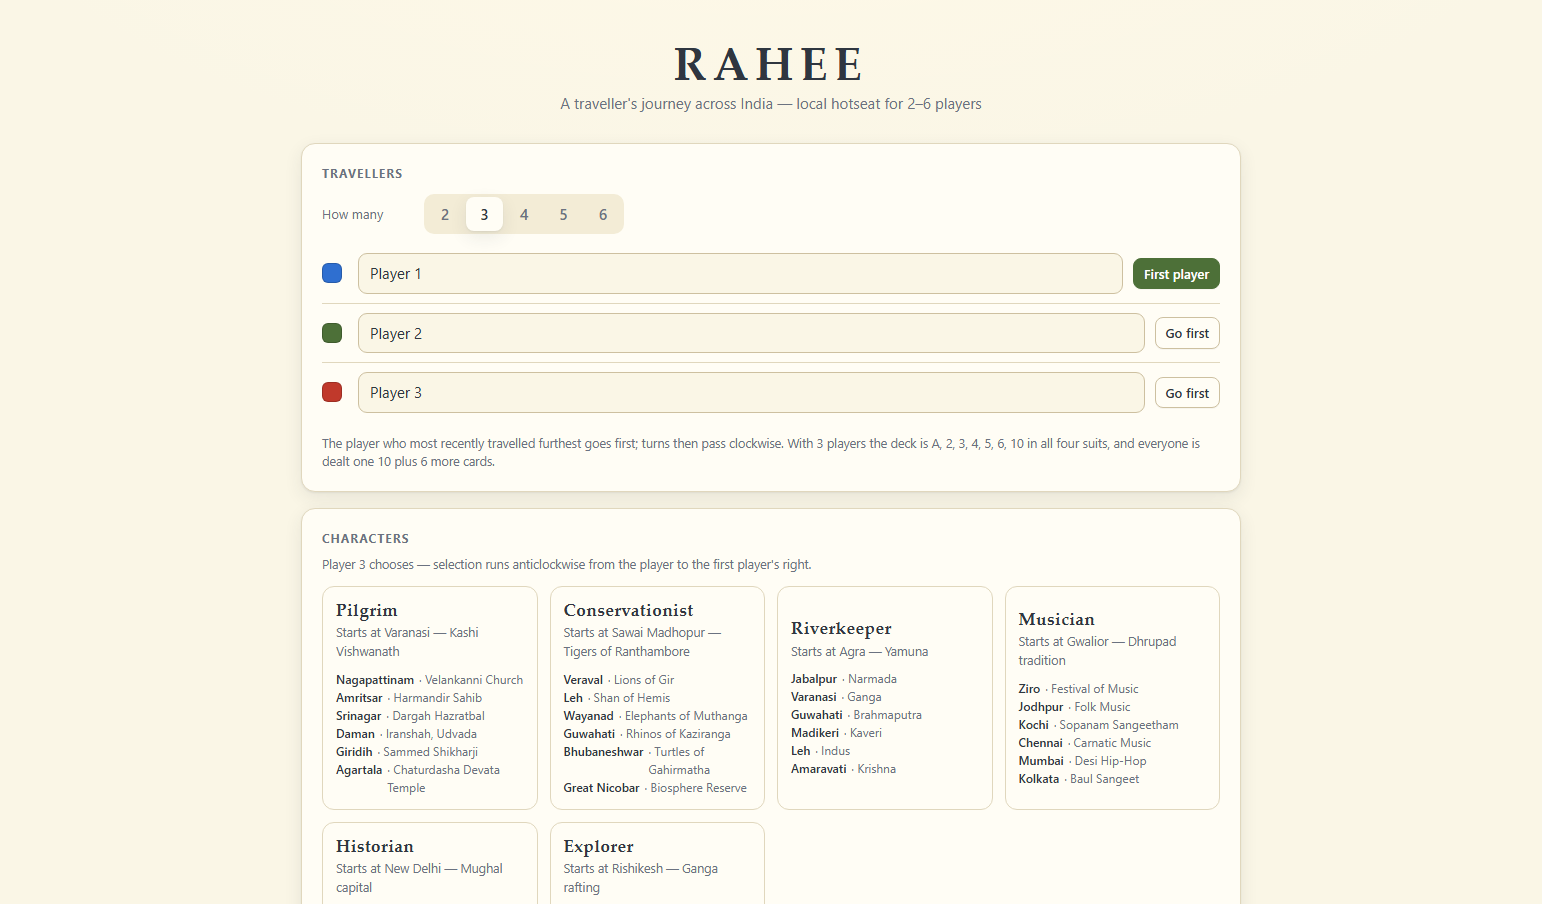
\includegraphics[width=0.8\textwidth]{shots/01-setup.png}
\end{center}
Screenshot of the application running in the browser (setup screen).

\subsection*{S3 --- Board data file}
A representative excerpt of the structured board data file (\texttt{data/board.json}), showing a city, a route and a character record:
\begin{verbatim}
{ "id": "new-delhi", "name": "New Delhi", "x": 663, "y": 687,
  "tourist": 1, "attraction": "Qutb Minar", "airport": true }

{ "from": "new-delhi", "to": "lucknow", "type": "flight",
  "steps": 1, "surcharge": 4000 }

{ "id": "pilgrim", "start": "varanasi",
  "goals": [ { "city": "amritsar", "blurb": "Harmandir Sahib" } ] }
\end{verbatim}
\placeholder{Optionally replace with a screenshot of data/board.json open in the editor}

\subsection*{S4 --- Rules engine structure}
Principal functions exported by the rules-engine module, showing its coverage of the rulebook: hand dealing, playing a card, computing legal movement, stepping and undoing a step, resolving a move (memories, tourism), starting/ending a road trip, laying road-trip cards, scoring a player, and computing final scores.
\placeholder{Optionally replace with a screenshot of the rules-engine source file}

\subsection*{S5 --- Automated test run}
\placeholder{PASTE SCREENSHOT HERE --- terminal output of the random-game test suite completing successfully}

\subsection*{S6 --- Turn flow across screens}
\begin{center}
  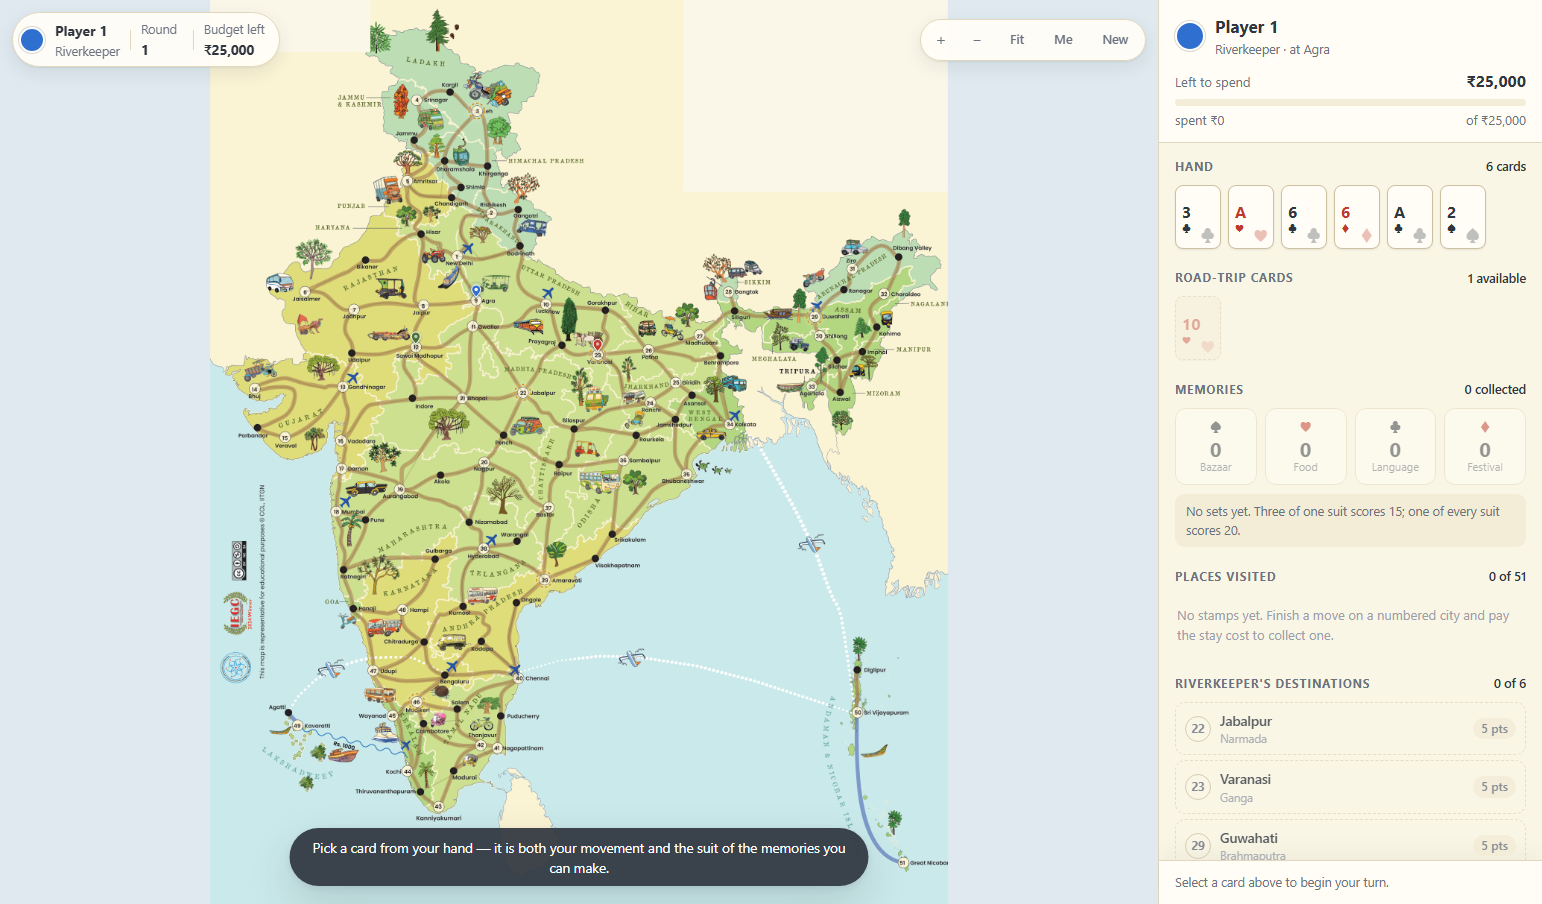
\includegraphics[width=0.8\textwidth]{shots/06-play-board.png}
\end{center}
The board/play screen mid-turn, reached via setup and the private handover screen.

\subsection*{S7 --- Sample game state / scoreboard}
\begin{center}
  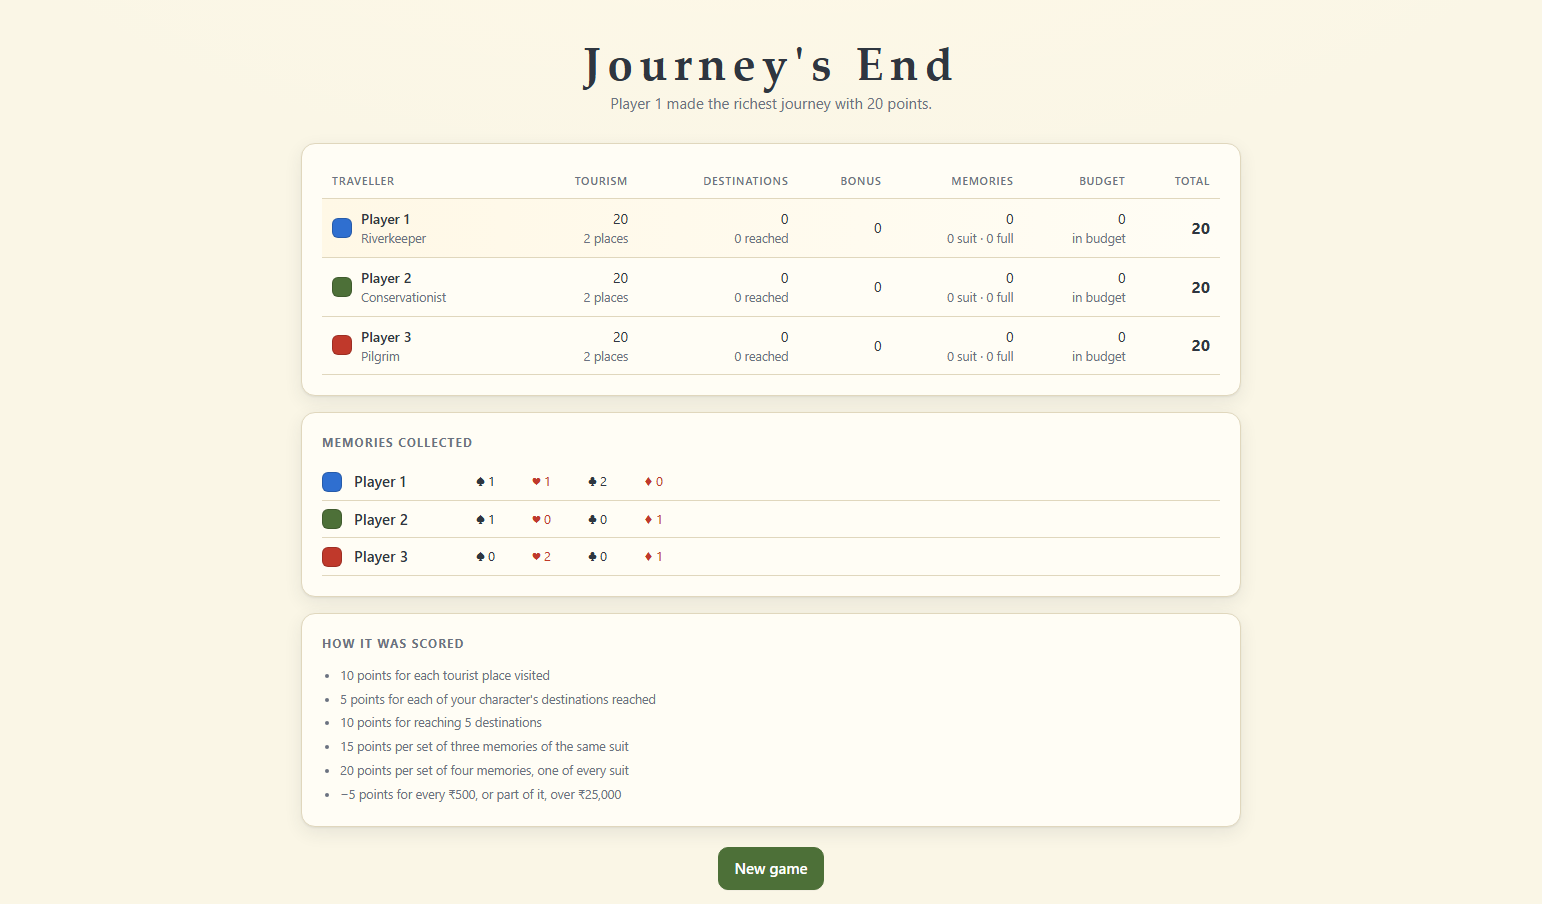
\includegraphics[width=0.8\textwidth]{shots/13-scoreboard.png}
\end{center}
The final scoreboard, with each player's score broken down into its scoring components.

\subsection*{S8 --- Strongest end-to-end evidence}
\begin{center}
  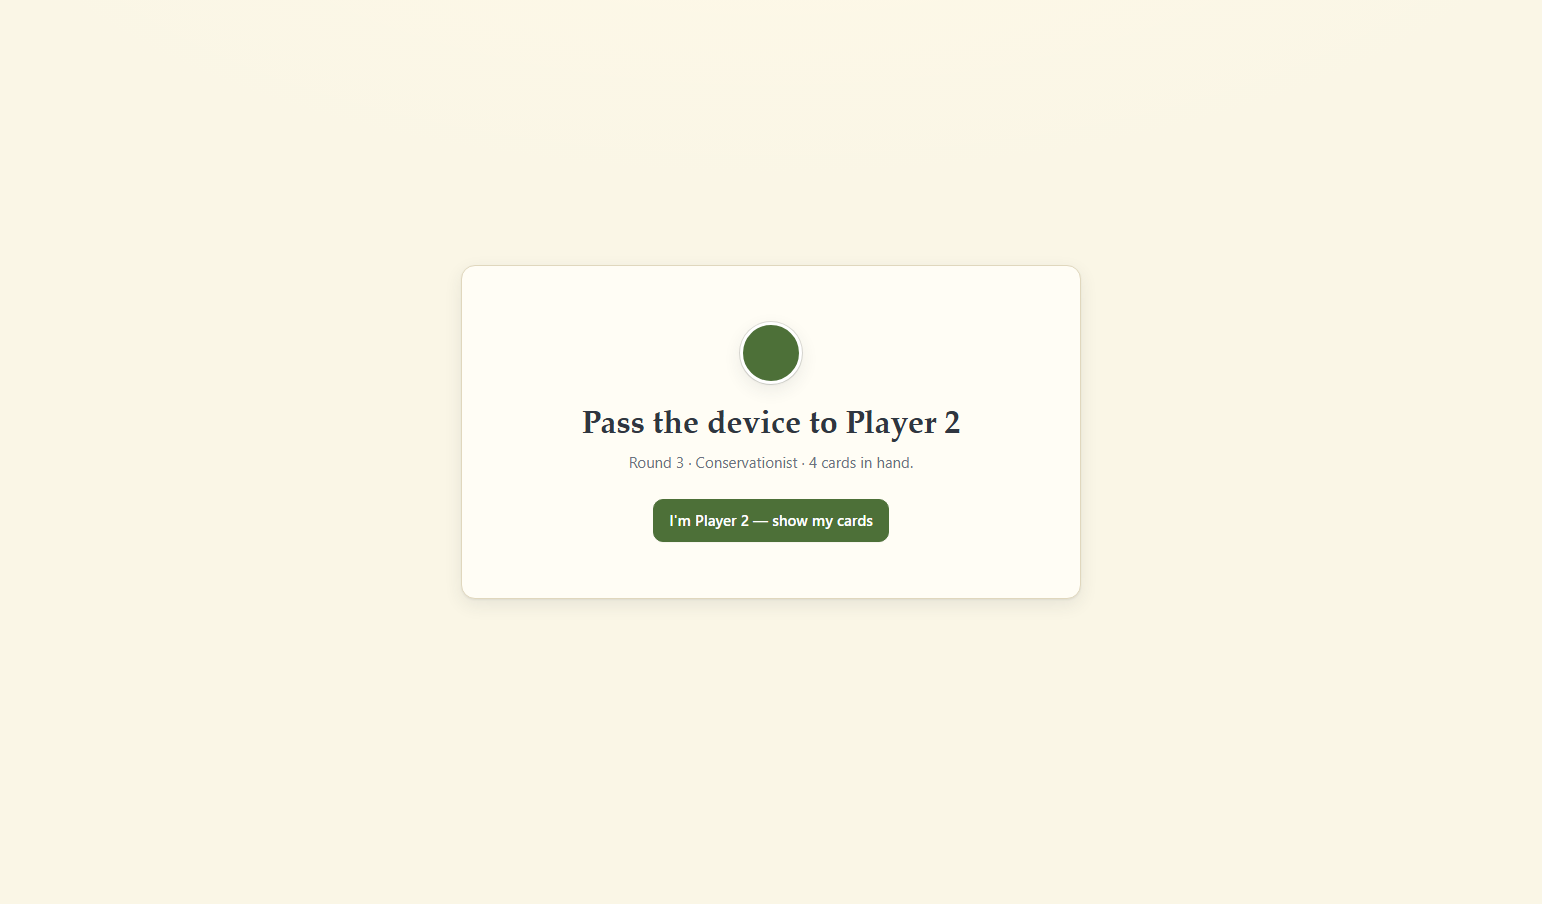
\includegraphics[width=0.8\textwidth]{shots/12-midgame.png}
\end{center}
A full game in progress: player actions taken through the interface, reflected correctly in budget, memories, visited places and token position.

\section{Tasks In Progress}

\begin{itemize}[leftmargin=1.4em]
  \item Implement the server process (room manager, authoritative rules engine, per-player state redaction).
  \item Implement the real-time connection layer between client and server (WebSocket messages for turns, movement, chat).
  \item Implement destination-based route planning: candidate-route computation within a card's remaining allowance, with waypoint selection, kept private to the active player and any road-trip invitees.
  \item Implement public and private chat.
  \item Implement room creation/joining by a short room code.
  \item Adapt the existing board rendering and turn-action UI to react to server-pushed state instead of local engine calls.
\end{itemize}

\section{Tasks Planned}

\begin{itemize}[leftmargin=1.4em]
  \item Reconnection handling (token-based rejoin after a dropped connection) and server-side save/resume.
  \item Responsive, touch-first layout for phones (board, sidebar, turn controls, chat).
  \item Continuous integration: linting, automated tests, and a security scan on every change.
  \item Deployment to a stateful hosting environment (the online version requires a persistent server process, unlike the current static-file prototype).
  \item AI players to fill empty seats (a later-phase requirement).
  \item Complete end-to-end multiplayer testing and QA defect tracking.
\end{itemize}

\section{Problems / Issues}

\begin{itemize}[leftmargin=1.4em]
  \item The connection data for the printed board (which cities join, route types, exact step counts and surcharges) has not yet been supplied by the client (CCL). Every route currently uses a placeholder value of one step, traced from the printed artwork, pending the official data.
  \item Any additional project issues should be added below as they occur.
\end{itemize}

\noindent Additional issue log:
\begin{itemize}[leftmargin=1.4em]
  \item \rule{0.82\linewidth}{0.4pt}
  \item \rule{0.82\linewidth}{0.4pt}
  \item \rule{0.82\linewidth}{0.4pt}
\end{itemize}

\section{Team Member Time --- Previous Week}

Replace the placeholders with the actual tasks and hours spent. Do not estimate unless the team agrees on the estimate.

\begin{tabularx}{\textwidth}{@{} l l Y l @{}}
  \toprule
  \textbf{Member} & \textbf{Name} & \textbf{Task(s)} & \textbf{Hours} \\
  \midrule
  Member 1 & Tanuj Sharma & \bracket{Task(s)} & \bracket{Hours} \\
  Member 2 & Sai Gawali & \bracket{Task(s)} & \bracket{Hours} \\
  Member 3 & Siddhesh Patil & \bracket{Task(s)} & \bracket{Hours} \\
  Member 4 & Mukesh Dewangan & \bracket{Task(s)} & \bracket{Hours} \\
  Member 5 & Kshitij Kasodkar & \bracket{Task(s)} & \bracket{Hours} \\
  \bottomrule
\end{tabularx}

\section{PoC Meeting}

\begin{tabularx}{\textwidth}{@{} l Y @{}}
  \toprule
  Last meeting date & \bracket{DD/MM/YYYY} \\
  Meeting mode & \bracket{Online / Offline} \\
  Key discussion / action items & \bracket{Enter 2--4 short points} \\
  \bottomrule
\end{tabularx}

\section{Current Build}

\begin{tabularx}{\textwidth}{@{} l Y @{}}
  \toprule
  Current build date & \bracket{Enter actual date --- must be within the last two days} \\
  Build / version identifier & \bracket{e.g. Git commit / branch / v0.1} \\
  Build status & \bracket{Working / Issues found / Under test} \\
  \bottomrule
\end{tabularx}

\section{Test Results on the Current Build}

The purpose of these tests is to verify the rules engine end to end through the interface. A test should be marked unsuccessful if the player cannot complete the intended action correctly through the interface, even when an individual engine function appears to work in isolation.

\begin{tabularx}{\textwidth}{@{} l Y l Y @{}}
  \toprule
  \textbf{Test ID} & \textbf{Test} & \textbf{Result} & \textbf{Actual result / notes} \\
  \midrule
  TC01 & Deal hands for the chosen player count & \bracket{Pass/Fail} & \bracket{Actual result} \\
  TC02 & Play a card and move along a legal route & \bracket{Pass/Fail} & \bracket{Actual result} \\
  TC03 & Earn a memory for efficient travel / meeting a traveller & \bracket{Pass/Fail} & \bracket{Actual result} \\
  TC04 & Visit a tourist place and mark its stamp & \bracket{Pass/Fail} & \bracket{Actual result} \\
  TC05 & Start and resolve a road trip & \bracket{Pass/Fail} & \bracket{Actual result} \\
  TC06 & Play an Ace in each of its three uses & \bracket{Pass/Fail} & \bracket{Actual result} \\
  TC07 & Detect the end-game trigger and complete the round & \bracket{Pass/Fail} & \bracket{Actual result} \\
  TC08 & Compute a final score with a correct breakdown & \bracket{Pass/Fail} & \bracket{Actual result} \\
  TC09 & Save and resume a game in progress & \bracket{Pass/Fail} & \bracket{Actual result} \\
  TC10 & Full single-device game walkthrough (headless browser) & \bracket{Pass/Fail} & \bracket{Actual result} \\
  \bottomrule
\end{tabularx}

\vspace{6pt}
\begin{tabularx}{0.6\textwidth}{@{} l Y @{}}
  Total tests & \bracket{Enter number} \\
  Unsuccessful tests & \bracket{Enter number} \\
  Successful tests & \bracket{Enter number} \\
\end{tabularx}

\section{QA Defects Found}

If no defects were found, write ``No defects found in this build.'' If defects exist, record them below.

\begin{tabularx}{\textwidth}{@{} l Y Y Y Y @{}}
  \toprule
  \textbf{Defect ID} & \textbf{Title} & \textbf{Steps / Condition} & \textbf{Expected} & \textbf{Actual / Status} \\
  \midrule
  \bracket{Enter} & \bracket{Enter} & \bracket{Enter} & \bracket{Enter} & \bracket{Enter} \\
  \bracket{Enter} & \bracket{Enter} & \bracket{Enter} & \bracket{Enter} & \bracket{Enter} \\
  \bracket{Enter} & \bracket{Enter} & \bracket{Enter} & \bracket{Enter} & \bracket{Enter} \\
  \bracket{Enter} & \bracket{Enter} & \bracket{Enter} & \bracket{Enter} & \bracket{Enter} \\
  \bottomrule
\end{tabularx}

\section{Remaining Screenshot Evidence}

\subsection*{S9 --- Server / real-time evidence}
Not yet implemented (see \S5). Leave blank until the server and WebSocket layer are in place.
\placeholder{PASTE SCREENSHOT HERE --- once implemented, a browser/terminal screenshot showing a real-time update reaching a second connected device}

\subsection*{S10 --- Test results}
\placeholder{PASTE SCREENSHOT HERE --- the completed test table above, once the current build's tests have been run}

\subsection*{S11 --- QA defects}
\placeholder{PASTE SCREENSHOT HERE --- the defect list, if defects are found}

\section{Weekly Summary}

This week's evidence establishes the completed foundation for RAHEE: a fully data-driven rules engine, tested against the official rulebook and its worked examples, with a complete single-device gameplay loop from setup through to a transparent final scoreboard. The main milestone reached is a working, rule-correct implementation of the physical game. The design for the next milestone --- a real-time, secure, multi-device online architecture, with the same rules engine running as the sole authority on a server, and public/private chat --- has been finalized and implementation has begun. The next reporting period is expected to cover the server process, the real-time connection layer, and the first cross-device play test.

\vspace{18pt}
\noindent Prepared by: \bracket{Team / Member Name}\\
Reviewed by: \bracket{PoC / Mentor Name}\\
Date: \bracket{DD/MM/YYYY}

\end{document}
